\section{Warum p2p?}
    Das vorausgegangene Projekt einer Verbindungskonfiguration von IoT-Geräten \linebreak \cite{aiProject} hat gezeigt, dass eine initiale p2p Verbindung aufgebaut werden muss, um eine Wi-Fi Verbindung konfigurieren zu können. In Verbindung mit einer ad-hoc Verbindung muss auch gleichzeitig eine Service Discovery betrachtet werden, um den initialen verbindungslosen Informationsaustausch über mögliche Verbindungspartner zu ermöglichen. Diese  findet aktuell ebenfalls über Wi-Fi Direct in Form von {\it DNS Service Discovery} statt. Dies hat den Vorteil, dass sich zusätzliche Daten mit einem einzigartigen Schlüssel dem Eintrag eines Service hinzufügen lassen. Eine p2p Technologie muss somit nicht zwingend verbindungslosen Beacon Signale mit Nutzdaten zur Verfügung stellen, da auch eine Hybridlösung genutzt werden kann. Das Erkennen von verfügbaren Services funktioniert bereits stabil über Wi-Fi Direct, somit wird im Weiteren lediglich der Aufbau einer p2p Verbindung thematisiert.
    
    Eine direkte Verbindung zwischen zwei Endgeräten ist nötig, wenn Daten zwischen Anwendungen ausgetauscht werden sollen und keine Verbindung über ein gemeinsames Netzwerk oder einen Server stattfinden kann oder soll. Mögliche Anwendungsfälle einer solchen p2p Verbindung sind oftmals die kabellose Nutzung von Peripheriegeräten oder der Austausch von Dateien ähnlich zu {\it Apple Air Drop}. Verbindungen zwischen Endgeräten ohne die Nutzung einer bestehenden Netzwerk-\linebreak infrastruktur resultiert in einer von der genutzten Technologie abhängigen, stark reduzierten Reichweite, welche zwischen den Geräten überwunden werden kann.
    
    Das Zustandsmodell \reffig{p2p:state} eines p2p Verbindungsaufbaus lässt sich aus Sicht der beteiligten Geräte soweit vereinfachen, dass lediglich fünf von außen beobachtbare Zustände für eine erfolgreiche Nutzung der Verbindung relevant sind. Damit der Nutzer beim Verbindungsaufbau lediglich in den Prozess mit seinem Smartphone interagieren muss, sollte der p2p Verbindungsaufbau seine Zustände so vereinfacht darstellen können, um einen konsistenten Ablauf automatisiert gewährleisten zu können.
    
    Zunächst soll über den Zustand {\it INACTIVE} erkannt werden können, wenn die zu verwendende Schnittstelle ausgeschaltet ist, um sie im Ablauf des Programms einschalten zu können. Sobald der Zustand {\it IDLE} erreicht ist, kann die Schnittstelle genutzt werden, um Verbindungen über {\it ACCEPTING} zu akzeptieren oder eine neue Verbindung zu einem anderen Gerät über {\it CONNECTING} aufzubauen. Sobald ein Gerät Verbindungen annimmt und ein weiteres Gerät versucht, sich zu diesem zu verbinden, wechseln beide Geräte im Erfolgsfall in den Zustand {\it CONNECTED} und besitzen einen gemeinsamen Kommunikationskanal. Sobald die Verbindung geschlossen wird, befinden sich beide Geräte wieder im Grundzustand {\it IDLE}. Falls eine Technologie mehr als eine parallele Verbindung erlaubt, teilt sich diese beim Akzeptieren einer neuen Verbindung auf und verbleibt weiterhin gleichzeitig im Zustand {\it ACCEPTING}.

    Ein besonderer Nutzungspunkt für p2p Verbindungen stellen IoT-Geräte dar, da so zum einen Kommunikation ohne Konfiguration des Nutzers zwischen den IoT-Geräten stattfinden kann und eine Konfiguration der IoT-Geräte durch den Nutzer stattfinden kann ohne Peripherie an das Gerät anschließen zu müssen. Internet of Things ist ein Sammelbegriff für Gebrauchsgegenstände wie Heizungsthermostate oder Maschinen wie CNC-Fräsen, die in einer moderneren Interpretation ihrer Funktionalität über ein Netzwerk untereinander und mit Servern kommunizieren. Anwendungsgebiete können die Hausautomation, Sensornetzwerke und Betriebsüberwachung von Maschinen sein. In einem weiter gefassten Blickfeld wird unter diesem Begriff auch die Vernetzung von ganzen Städten und deren Infrastruktur untersucht \cite{ituGroup}.
    
    \begin{figure}[ht]
         \centering
	      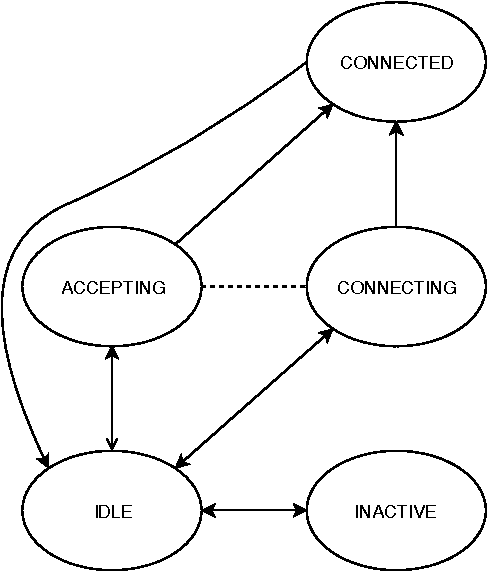
\includegraphics[width=0.5\textwidth]{p2p-State.pdf}
    	   \caption[Zustandsmodell eines p2p Verbindungsaufbaus]{Das Zustandsmodell eines p2p Verbindungsaufbaus zeigt die von außen beobachtbaren Zustände für eine erfolgreiche Nutzung einer p2p Verbindung. } \label{p2p:state}
	\end{figure}       
    
    \subsection{Services}
    Für solche IoT-Geräte muss eine Erstkonfiguration initial vorgenommen werden, um eine Kommunikation mit anderen Geräte zu ermöglichen. Da nicht jedes Gerät einen Bildschirm oder komplexe Eingabemöglichkeiten besitzt, ist es sinnvoll, diese Einrichtung auf ein Smartphone auszulagern, wie es bereits im vorausgegangenen Projekt geschehen ist. Da die Konfiguration durch einen REST-Server angeboten wird, ist es so auch möglich, weitere Konfigurationsmöglichkeiten für Sensoren und Aktuatoren als weiteren Service anzubieten.
    
    Ein Service definiert sich als ein Dienst, welcher Anderen eine Leistung oder Aufgabe bereitstellt. Im Sinne der Informatik ist ein solcher Dienst eine Einheit von Programmen, welche durch eine Schnittstelle eine Funktionalität verwaltet und extern zur Verfügung stellt. Eine solche Schnittstelle kann auf verschiedene Arten bereitgestellt werden, jedoch sollten diese Schnittstellen über Verträge abgesichert werden, um ungewollte Änderungen im Betrieb zu vermeiden und eine reibungslose Anbindung von neuen Funktionalitäten zu gewährleisten \cite[S.11]{finger}.
    
    Im Rahmen einer Anwendungsarchitektur als Sammlung von {\it Microservices} treten Services als {\it Messagehandler} auf und definieren ihre Schnittstellen durch Nachrichten oder {\it RPC} Aufrufe. Microservices können dabei wiederum als Services betrachtet werden. Vorteile bietet eine solche Architektur in einer leichten Skalierbarkeit der Anwendung oder einzelner Teile und einer sauberen Kapselung von Anwendungs-teilen. Zwischen {\it Messagehandlern} wird oftmals auf Authentifizierung verzichtet, wenn die teilnehmenden Dienste bekannt sind, da auf diese Weise ein höherer Durchsatz erzielt werden kann \cite{microservices}.
    
    Ein {\it Daemon}, welcher eine Hardwarekomponente verwaltet, kann ebenfalls als Service, welcher abstraktere Funktionalität auf dieser Hardware bereitstellt, definiert werden. Auf diese Kategorie von Services trifft die Einschränkung der Einzigartigkeit zu, da immer eine Systemresource nur von einem Programm genutzt werden kann.
    
    Im simpelsten Fall kann ein Service auch als Server definiert werden, um seine Funktionalität Clients zur Verfügung zu stellen. Dies bietet sich besonders dann an, wenn verschiedene Architekturen von Clients in einer hohen Anzahl den selben Service benutzen sollen oder Clients zunächst eine Authentifizierung vornehmen sollen. 
    Ein klassisches Client/Server-Modell sieht hierbei vor, dass auszuführende Berechnungen so aufgeteilt werden, dass ein Server Daten konsistent nutzen kann und in der Lage ist, die verwalteten Daten mehreren Clients auszuliefern \cite[S.8]{abts}.
        
%    \subsection{Servicestabilität (Todo: entfällt eventuell)}
%    - API Versionierung
    
%    - Absichern von Änderungen durch Contract-Driven-Development
    
%    - Integrationstests
    \subsection{Netzwerktopologie}
    
    Der Begriff {\it peer-to-peer} beschreibt eine Art von infrastrukturlosen Netzwerk zwischen zwei oder mehr lokalen Geräten. Um die Vor- und Nachteile einer solchen Verbindung darstellen zu können, werden zunächst die unterschiedlichen Netzwerktypen gegenüber gestellt. Ebenso ist es sinnvoll die zu evaluierenden Technologien in verschieden Topologien einzuordnen, um sie im Hinblick auf Reichweiten und Eigenschaften vergleichen zu können.
    
    {\it Ad Hoc} Netzwerktechnologien erlauben es zwei oder mehr Geräten ein dezentrales Netzwerk aufzubauen. Um die Kontrolle über die gemeinsame Schnittstelle zu erlangen, agiert hierbei entweder eines der Geräte als Verwalter der Verbindung oder es werden spezielle Sequenzen zum Frequenzwechsel in Verbindung mit einer Kollisionsauflösung durch zufällig langes Warten definiert, um Kommunikations-\linebreak konflikte zwischen Teilnehmern zu vermeiden.
    
    Im Gegensatz zum dezentralisierten {\it ad hoc} Netzwerk nutzt ein Stern-basiertes Netzwerk Knotenpunkte, um die Kommunikation zu Endgeräten zu übernehmen. Wi-Fi bildet ein solches Netzwerk mit {\it Access Points} ab, da diese ein gemeinsames Übertragungsmedium aller verbundenen Endgeräte verwalten und keine Endgeräte direkt miteinander kommunizieren. Ein solches Netzwerk ist dann sinnvoll, wenn der Übergang zu einem anderen Netzwerk in einer Singularität verwaltet werden soll und Endgeräte generell wenig untereinander kommunizieren, da eine Datenübertragung so die doppelte Bandbreite benötigt, um die selbe Übertragungsgeschwindigkeit zu erzielen, da Pakete zunächst zum Knotenpunkt übertragen werden und dieser die Pakete über das gemeinsame Medium erneut an das Zielgerät übermittelt.

    Alle zu überprüfenden Technologien bilden ein {\it ad hoc}, da das Ziel ist, das IoT Gerät erst in ein Wi-Fi Netzwerk zu bringen und somit noch keine gemeinsame Netzwerkverbindung besteht. Relevant ist auch, dass lokale Geräte in einem Raum angesprochen werden können, ohne große Distanzen überbrücken zu müssen. Die genutzten Technologien gehören unterschiedlichen Topologien an, wodurch sich ihre Einsatzgebiete auch unterscheiden:
    \begin{itemize}
    \item {\it Wi-Fi Direct} ist ein Wireless Local Area Network (WLAN) und kann in dieser Kategorie über theoretische Distanzen von bis zu 100 Metern Daten übertragen. Ähnlich zu Wi-Fi ist die Signalstärke von Wi-Fi Direct ausrei-chend, um in einem Gebäude eine Verbindung zu anderen Geräten aufbauen zu können. Da Signale stark durch Objekte und Wände gedämpft werden, reduziert sich jedoch die Reichweite innerhalb von Gebäuden drastisch wodurch eine Einordnung als Personal Area Network (PAN) zutreffender ist.
    
    \item {\it Bluetooth} ordnet sich ebenfalls als PAN ein und erlaubt den Datenaustausch bis zu einer theoretischen Distanz von 10 Metern. Dies ist ausreichend, um Geräte im Bereich um die eigene Person anzusteuern, was eine durchschnittliche Raumgröße abdeckt. Bluetooth unterstützt eine Vielzahl von Protokollen, insbesondere zur Audioübertragung. Typische Anwendungsfälle sind hierbei drahtlose Peripheriegeräte und der lokale Dateienaustausch.
    
    \item {\it NFC} kann lediglich Distanzen von unter 10 Zentimetern überbrücken, und kommt so größtenteils in Verbindung mit mobilen Zahlungsmitteln zum Einsatz. NFC ist zum einen der Name der eingesetzten Technologie als Weiter-führung von RFID, gleichzeitig beschreibt es jedoch auch eine Netzwerktopologie, die es Geräten erlaubt auf einem engen Raum miteinander zu kommunizieren. 
    
    \item {\it USB} ist ein kabelgebundenes Übertragungsmedium und erfordert so einen direkten Zugang zum Raspberry Pi. Da in der Spezifikation zu USB 2.0 eine maximale Kabellänge von 5 Metern definiert ist \cite{usbSpec}, ordnet sich dieser Standard ebenfalls als PAN ein.
    
    \end{itemize}